\subsection{Расчет рыночной стоимости ТС}


\par \indent Рыночная стоимость транспортного средства - наиболее вероятная стоимость, по которой транспортное средство может быть отчуждено на открытом рынке в условиях конкуренции, когда стороны сделки действуют разумно, располагая всей необходимой информацией, а на величине стоимости сделки не отражаются какие-либо чрезвычайные обстоятельства [4]. Рыночная стоимость транспортного средства  рассчитывается  для условий конкретных товарных рынков транспортных средств, соответствующих месту государственной регистрации транспортного средства потерпевшего.
\par Определение рыночной стоимости ТС может производится сравнительным и затратным подходом, а именно:  сравнительный анализ продаж (анализ информации о первичном и вторичном рынке АМТС в Российской Федерации);  затратный (с учетом износа АМТС).
\par В оценочной практике наиболее распространенным и предпочтительным является метод прямого сравнения продаж, в соответствии с которым стоимость объекта оценки определяется как средняя цена отобранных аналогов с последующими параметрическими и износными корректировками.   В цены аналогов не вносятся корректировки, если аналоги являются идентичными и равновозрастными объектами по отношению к объекту оценки. 
\par Общий алгоритм метода прямого сравнения продаж:
\begin{list}{-}{}
	\item сбор необходимой информации об объектах;
	\item  производится выборка цен на объекты;
\item  проверка полученной выборки на однородность путем расчета коэффициента вариации;
\item  при значении коэффициента вариации, не превышающем 20\%, определяется средняя цена, которая принимается за стоимость объекта [9]
\item  при превышении коэффициента вариации значения  20\%  выборка исследуется на наличие выбросов с использованием метода Граббса [9,10].
\end{list}
Рыночная стоимость ТС отражает его комплектацию, комплектность, фактическое техническое состояние, срок эксплуатации, пробег, условия, в которых оно эксплуатировалось, коньюктуру первичного и вторичного рынка ТС в регионе. В общем случае расчет рыночной стоимости производится по формуле:
\begin{equation}\label{eq:aa}
C_{\text{КТС}} = C_{cp}\left(1 \pm  \left( \frac{\text{П}_{\text{П}}}{100}\right) \pm\left( \frac{\text{П}_{\text{Э}}}{100}\right) \right) + C_{\text{ДОП}}, \text{руб}
\end{equation}

\noindent где: $C_\text{ср}$ -- средняя цена ТС, \text{руб};\\
$ \text{П}_\text{П}$ -- процентный показатель корректировки средней цены ТС по пробегу, \%;\\
$ C_\text{ДОП}$ -- дополнительное увеличение (уменьшение) стоимости в зависимости от его комплектации, наличия повреждений и акта их устранения, обновления составных частей, руб.\\
Корректировка средней цены ТС, исходя из его комплектности, опций комплектации, обновления составных частей, повреждений и акта их устранения определяется по формуле:
\begin{equation}\label{eq:b}
  C_\text{ДОП}=C_1\pm C_2\pm\left( C_P+C_M+C_\text{ЗЧ}\cdot\left( 1-\text{И}\right) +C_\text{УТС}\right), \text{руб}  
\end{equation} 
где:\\
$C_1$ --увеличение средней цены транспортного средства вследствие замены (обновления его частей в процессе эксплуатации, руб;\\
$ C_2$ -- изменение средней цены транспортного средства в зависимости опций его комплектации, руб;\\
 $ C_P $ -- стоимость ремонтных работ, руб;\\
 $C_M$--  стоимость материалов, руб;\\
 $C_\text{ЗЧ}  $ -- стоимость запасных частей, руб;\\
 $ C_\text{УТС} $ -- величина УТС, руб;\\
 $ \text{И} $ -- величина износа, \%;\\
 
Приоритетным способом определения рыночной стоимость TC
является метод сравнительного подхода, основанный на объективных справочных данных о ценах на подержанные автомобили  в регионе, где проводится оценка.
   
При определении стоимости транспортного средства сравнительным подходом экспертом были использованы  Интернет-источники сведений об аналогах (таблица \ref{tab:5}), содержащие краткое описание основных характеристик и технического состояния. 
 
\begin{longtable}{|p{5mm}|p{85mm}|c|p{60mm}|l|}
	\caption[]{\footnotesize {Описание ТС, идентичных оцениваему}} \label{tab:5}\\ 
	\hline
	%\rowcolor[HTML]{C0C0C0} 
	\rowcolor[HTML]{EFEFEF}
\bf	\text{n/n} &\bf  Описание аналога & \bf URL-адрес преложения  \\ \hline \endhead
		\toprule \centering
\Rownum  &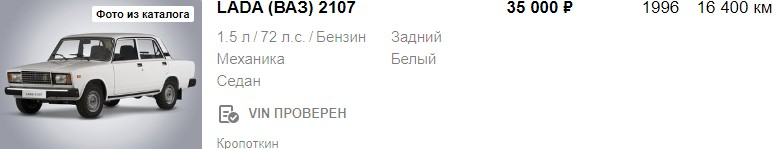
\includegraphics[width=0.99\linewidth]{A_1} &{\noindent \scriptsize\ \url {https://auto.ru/krasnodar/cars/vaz/2107/1996-year/all}} \\ \hline 	\centering
%	\rowcolor[HTML]{EFEFEF} 
\Rownum  &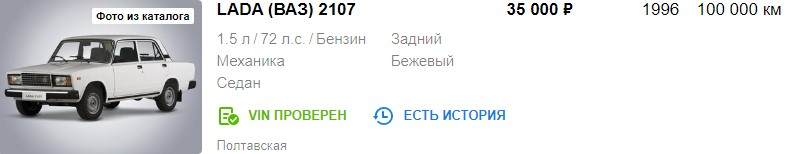
\includegraphics[width=0.99\linewidth]{A_2} & {\noindent \scriptsize\ \url {https://auto.ru/krasnodar/cars/vaz/2107/1996-year/all}} \\ \hline 	\centering
\Rownum  &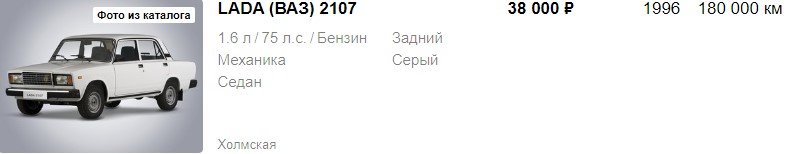
\includegraphics[width=0.99\linewidth]{A_3} &{\noindent \scriptsize\ \url {https://auto.ru/krasnodar/cars/vaz/2107/1996-year/all}} \\ \hline 	\centering
\Rownum  &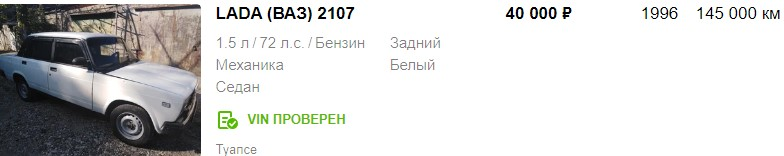
\includegraphics[width=0.99\linewidth]{A_4} &{\noindent \scriptsize\ \url {https://auto.ru/krasnodar/cars/vaz/2107/1996-year/all}} \\ \hline 	\centering
\Rownum &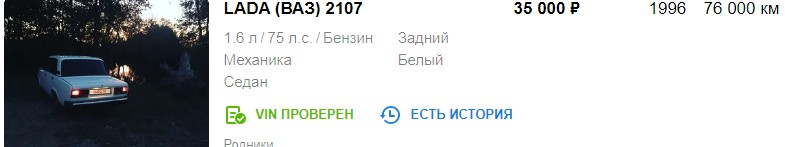
\includegraphics[width=0.99\linewidth]{A_5} &{\noindent \scriptsize\ \url {https://auto.ru/krasnodar/cars/vaz/2107/1996-year/all}} \\ \hline 	\centering
\Rownum  &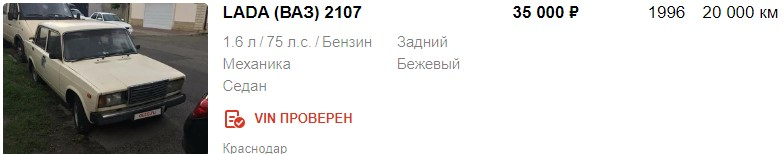
\includegraphics[width=0.99\linewidth]{A_6} &{\noindent \scriptsize\ \url {https://auto.ru/krasnodar/cars/vaz/2107/1996-year/all}}\\ \hline 	\centering
\Rownum  &
\includegraphics[width=0.99\linewidth]{A_7} &{\noindent \scriptsize\ \url {https://krasnodar.drom.ru/data/2107/35131847}} \\ \hline 	\centering
%\Rownum  &
\includegraphics[width=0.99\linewidth]{A_8} &{\noindent \scriptsize\ \url {https://https://krasnodar.drom.ru/lada/2107/34429407}} \\ \hline 	\centering \textbf{}
\Rownum &
\includegraphics[width=0.99\linewidth]{A_9} &{\noindent \scriptsize\ 
\url {https://krasnodar.drom.ru/lada/2107/33456928}} \\ \hline
					
\end{longtable}
%}

%	1. Определяется \overline{X} – среднее значение цены в %промежуточной выборке по формуле:        
 %
%где n – объем выборки (количество элементов в выборке);
%X_i – цена\  i– го объекта-аналога в промежуточной выборке.
%
%	2. Проверяется полученная выборка на однородность путем расчета %коэффициента вариации. Степень однородности выборки оценивается по %коэффициенту вариации (VB ), измеряющему  рассеивание данных %относительно среднего значения:
%V_B=\frac{\sigma_1}{\overline{X}}100%,  
%где \sigma_1- среднеквадратическое (или стандартное) отклонение, %определяемое по формуле:
%\sigma_1=\sqrt{\frac{\sum_{i=1}^{n}{{(X}_i-\overline{X})}^2}{n-1}};
%D= \frac{\sum_{i=1}^{n}{{(X}_i-\overline{X})}^2}{n-1}, где D -%дисперсия выборки.
	%Для малой выборки принято считать, что если VB <15%, то %однородность выборки высокая; 15% <VB<<25%, однородность выборки %средняя,  25% < VB< 33% однородность выборки низкая [9].
	%4. .При значении коэффициента вариации, не превышающем 20%, %определяется средняя цена, которая принимается за стоимость объекта.
	%5.  При превышении коэффициента вариации значения  20%  выборка %исследуется на наличие выбросов с использованием метода Граббса.
	%Окончательно, рассчитанная средняя цена предложения корректируется %с учетом торга в зависимости  от активности рынка – чем выше %спрос/предложение, тем ниже корректировка на торг. Для данного ТС %наиболее вероятное значение корректировки – 10.9% (данные %аналитического агентства «Автостат» %%http://www.autostat.ru/news/20083/)











%%%%%%%%%% среднеквадратичное отклонение и дисперсия выборки
%где $ \sigma_1 $- среднеквадратическое (или стандартное) отклонение, определяемое по формуле:
%\begin{equation}\label{ab}
%\sigma_1=\sqrt{\frac{\sum\limits_{i=1}^{n}{{(X}_i-\overline{X})}^2}{n-1}}
%\end{equation}
%
%\begin{equation}\label{ac}
%D= \frac{\sum\limits_{i=1}^{n}{{(X}_i-\overline{X})}^2}{n-1}
%\end{equation},
%
%
%где $ D $ -дисперсия выборки.
%Для малой Для малой выборки принято считать, что если VB <15\%, то однородность выборки высокая; 15\% <$  V_B  $<<25\%, однородность выборки средняя,  25\% < VB< 33\% однородность выборки низкая 
%
%4. .При значении коэффициента вариации, не превышающем 20\%, определяется средняя цена, которая принимается за стоимость объекта.
%5.  При превышении коэффициента вариации значения  20\%  выборка исследуется на наличие выбросов с использованием метода Граббса.
%6.	Окончательно, рассчитанная средняя цена предложения корректируется с учетом торга в зависимости  от активности рынка – чем выше спрос/предложение, тем ниже корректировка на торг. Для данного ТС наиболее вероятное значение корректировки – 10.9\% (данные аналитического агентства «Автостат» http://www.autostat.ru/news/20083/)
%
%\par Рыночная стоимость ТС  учитывает его фактическое техническое состояние, условия, в которых оно эксплуатировалось.
% Ремонт кузовных составляющих транспортного средства является фактором, влияющим на уменьшение средней цены ТС. В соответствии с Методикой [1], Приложение 3.3 <<Процентный показатель корректирования средней цены КТС в зависимости от условий эксплуатации>>, Таблица 1, для автомобилей со сроком эксплуатации до 7 лет, при восстановлении трех и больше кузовных составных частей уменьшение рыночной стоимости составляет 10 \%. 

%\par При определении стоимости транспортного средства сравнительным подходом экспертом использованы  Интернет-источники сведений об аналогах (Таблица \ref{tab:5}), содержащие краткое описание основных характеристик и технического состояния. Поскольку при определении рыночной стоимости  эксперту-технику данные о техническом состоянии и условиях эксплуатации не заданы и объективно не могут быть  получены при осмотре ТС на момент исследования, то для расчета принимается следующее:
%\begin{list}{-}{}
%	\item техническое состояние ТС соответствует сроку эксплуатации;
%	\item тс не эксплуатировалось в режиме такси или специальных условий эксплуатации;
%	\item фактический пробег ТС на момент повреждения составлял 45 513 км;
%	\item  29.06.2018 г. ТС \тс \, участвовал в ДТП, в результате которого  автомобиль получил механические повреждения задней правой двери, заднего правого порога, заднего правого колеса,  подушки SRS справа.
%\end{list}

%Из открытых банков данных полиции следует, что автомобиль с VIN: \,  \вин\,  как минимум дважды становился участником ДТП.
%Первый раз 29.06.2018  06:40, извещение о ДТП № 030046913, в котором автомобиль получил повреждения задней правой двери, заднего правого порога, заднего правого колеса, подушки SRS справа, Рис. \ref{ris:images/d1} и второй раз 22.05.2019 06:50, извещение о ДТП № 030034947, в котором автомобиль получил повреждения деталей передней левой и задней частей кузова, Рис. \ref{ris:images/d2}.
%%
%\vspace{\baselineskip}
%%
%\begin{figure}[H]\centering
%	\parbox[t]{0.49\textwidth}
%	{\centering
%		
\includegraphics[width=.49\textwidth]{images/d1}
%		\caption{\footnotesize {Повреждения в ДТП 29.06.2018 }}
%		\label{ris:images/d1}}
%	\hfil \hfil%раздвигаем боксы по горизонтали 
%	\parbox[t]{0.49\textwidth}
%	{\centering
%		
\includegraphics[width=.49\textwidth]{images/d2}
%		\caption{\footnotesize {Повреждения в ДТП 22.05.2019}}
%		\label{ris:images/d2}}
%\end{figure}
%%
%\vspace{\baselineskip}
%
%{\noindent  \footnotesize \tikz \fill [red] (1,0.5) rectangle (0.1,0.1); --{\footnotesize  Вмятины, вырывы, заломы, перекосы, разрывы и другие повреждения с изменением геометрии элементов (деталей) кузова и эксплуатационных характеристик ТС.}\\
%	\tikz \fill [yellow] (1,0.5) rectangle (0.1,0.1); --  {\footnotesize Повреждения колёс (шин), элементов ходовой части, стекол, фар, указателей поворота, стоп-сигналов и других стеклянных элементов (в т.ч. зеркал), а также царапины, сколы, потертости лакокрасочного покрытия или пластиковых конструктивных деталей и другие повреждения без изменения геометрии элементов (деталей) кузова и эксплуатационных характеристик ТС.}\\[1mm]
%	
%\renewcommand\baselinestretch{1.2}\small\normalsize

%\par Вследствие вышеизложенного коэффициент $ C_\text{ДОП}$ принимается равным -10 \%, коэффициенты $ \text{П}_{\text{Э}} $ и $ \text{П}_{\text{П}} $ принимаем равными нулю.

Средняя цена  $C_\text{ср}$  определяется на базе  средней рыночной цены продажи совокупности идентичных ТС на дату оценки: 
\begin{equation}\label{C}
C_\text{ср} =   \frac{ \sum\limits_{i=1}^n{C_i}}{n}
\end{equation}
 $C_\text{ср} =(\sum\limits_{i=1}^n{C_i})/n= (35000+35000+38000+40000+35000+35000+40000+33000)/8 =36 375 $, руб.\\
\noindent где: $ C_i $ - цена предложения к продаже i-го ТС, \\
\indent i - количество предложений, i=8.
\par Поскольку используемая выборка состоит из цен предложений к продаже, то для приведения к средней рыночной цене покупки применяется коэффициент торга $ K_T $, значение которого согласно данных аналитического агентства «Автостат» http://www.autostat.ru/news/20083/, %рис. \ref{fig:avtostat} 
\, составляет 5 \%. Соответственно, средняя цена предложений должна быть скорректирована в соответствии с нижеприведенной формулой \ref{Cp}:
\begin{equation}\label{Cp}
C_\text{ср} =  \left( \sum\limits_{i=1}^n{C_i}\right)  \cdot K_T , \,\, \text{руб}
\end{equation}
%%%%%%%%%%%%%%%%%%%%%  График АВТОСТАТ (если нужно)
%\begin{figure}
%	\centering
%	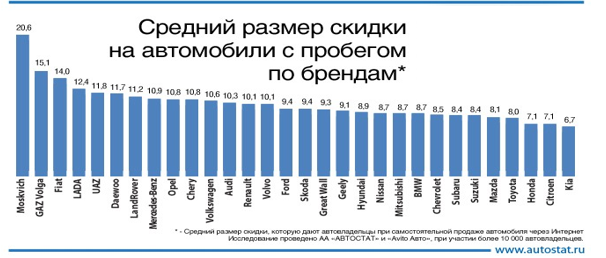
\includegraphics[width=0.7\linewidth]{images/avtostat}
%	\caption{График аналитического агентства <<Автостат>> процента уторговывания по маркам автомобилей}
%	\label{fig:avtostat}
%\end{figure}
Тогда,\,\, рыночная стоимость $ C $ автомобиля \тс \, с учетом торга и факторов, влияющих на рыночную стоимость составляет: 
\begin{equation}\label{cp}
C = C_\text{ср} \cdot  K_T 
%-  C_\text{ДОП} 
= 36375 \cdot(100-5)
%)\cdot 0.9 
=  34556 \, \, \text{руб},
\end{equation} 
\noindent что с учетом округления составляет 35000  рублей.

\par Таким образом, рыночная стоимость ТС \тс, \, с учетом всех имеющихся сведений о состоянии ТС на момент повреждения \датадтп\,  составляет 35000 (Тридцать пять тысяч) рублей.

%\paragraph*{} Федеральным законом от 25.04.2002 года № 40-ФЗ «Об обязательном страховании гражданской ответственности владельцев транспортных средств» в редакции на момент заключения договоров страхования и страхового случая (далее – Закон об ОСАГО) установлено:
%(пункт 18 статьи 12) что размер подлежащих возмещению страховщиком убытков при причинении вреда имуществу потерпевшего определяется: \par а) в случае полной гибели имущества потерпевшего - в размере действительной стоимости имущества на день наступления страхового случая за вычетом стоимости годных остатков. Под полной гибелью понимаются случаи, при которых ремонт поврежденного имущества невозможен либо стоимость ремонта поврежденного имущества равна стоимости имущества на дату наступления страхового случая или превышает указанную стоимость.\par Настоящим исследованием установлено, что стоимость восстановительного ремонта ТС \тс \, превышает рыночную стоимость ТС на момент повреждения. Таким образом, при определении стоимости восстановительных расходов необходимо произвести расчет стоимости годных остатков ТС.
%\par  
%Положением Банка России от 19 сентября 2014 г. N 432-П "О единой методике определения размера расходов на восстановительный ремонт в отношении поврежденного транспортного средства <<Глава 5. Порядок расчета стоимости годных остатков в случае полной гибели транспортного средства>> установлен алгоритм расчета годных остатков ТС.



